% !TeX root = ../main.tex
% Add the above to each chapter to make compiling the PDF easier in some editors.

\chapter{Introduction}
Real-time rendering is by no means a new research topic. Naturally developers and researchers have devised shortcuts and optimizations in both hardware and software as far back as the first applications in video games, visualization - scientific or otherwise - and simulation. There are methods and algorithms for almost any type of hardware, rendering technique and application scope. 
One more recently resurged trend is virtual reality (VR). The realization of comparably affordable, comfortable and hassle-free virtual reality headsets like the Oculus Rift series, the HTC Vive, Windows Mixed Reality design or the recently launched Valve Index led to a newfound vigor for the technology among consumers. Similarly, businesses as well as scientists are increasingly looking to VR for various fields of research, marketing opportunities, engineering support and more. \\
However, virtual reality poses challenges and requirements not commonly seen with traditional real-time applications on monoscopic screens. And while goals such as stable motion tracking and low latency, high performance rendering are as old as early VR HMDs, this recent resurgence has prompted much more active search for possible solutions. Among these requirements is the need for high framerates to give the user a better feeling of visual fluidity and to avoid motion sickness. VR applications need not only render at high framerate, they also need to do so at higher resolutions than common flat screens. As the much lower viewing distance and added lens distortion means pixels appear much larger to the user, the only way to combat visual aliasing and the so called screen door effect is to significantly increase pixel count and density. \\

Similarly to the opening example of \cite{InigoQuilez.2017}, let's assume a traditional console video game running at Full HD resolution and 60 frames per second, a common sight for 8th generation consoles. Meanwhile the same game running in a VR headset may require resolutions and framerate ranging from 1200 pixels per axis per eye (\autoref{fig:VR_HMD_res}) at 90 frames per second for entry level headsets up to or even exceeding 2000 pixels per axis per eye at 120 frames per second for high end devices like the Pimax 4K - not to mention image warp commonly requires an even higher internal rendering resolution by a factor of around 20\% or more. In the entry level case that means a resolution increase of roughly 1.6x and a framerate increase of 1.5x for a combined 2.4x power requirement compared to the console baseline, while in the high end case it is roughly 4.6x resolution and 4x framerate uptick for a combined 9.2x power requirement in comparison. \\

\begin{figure}[htb]
  \centering
  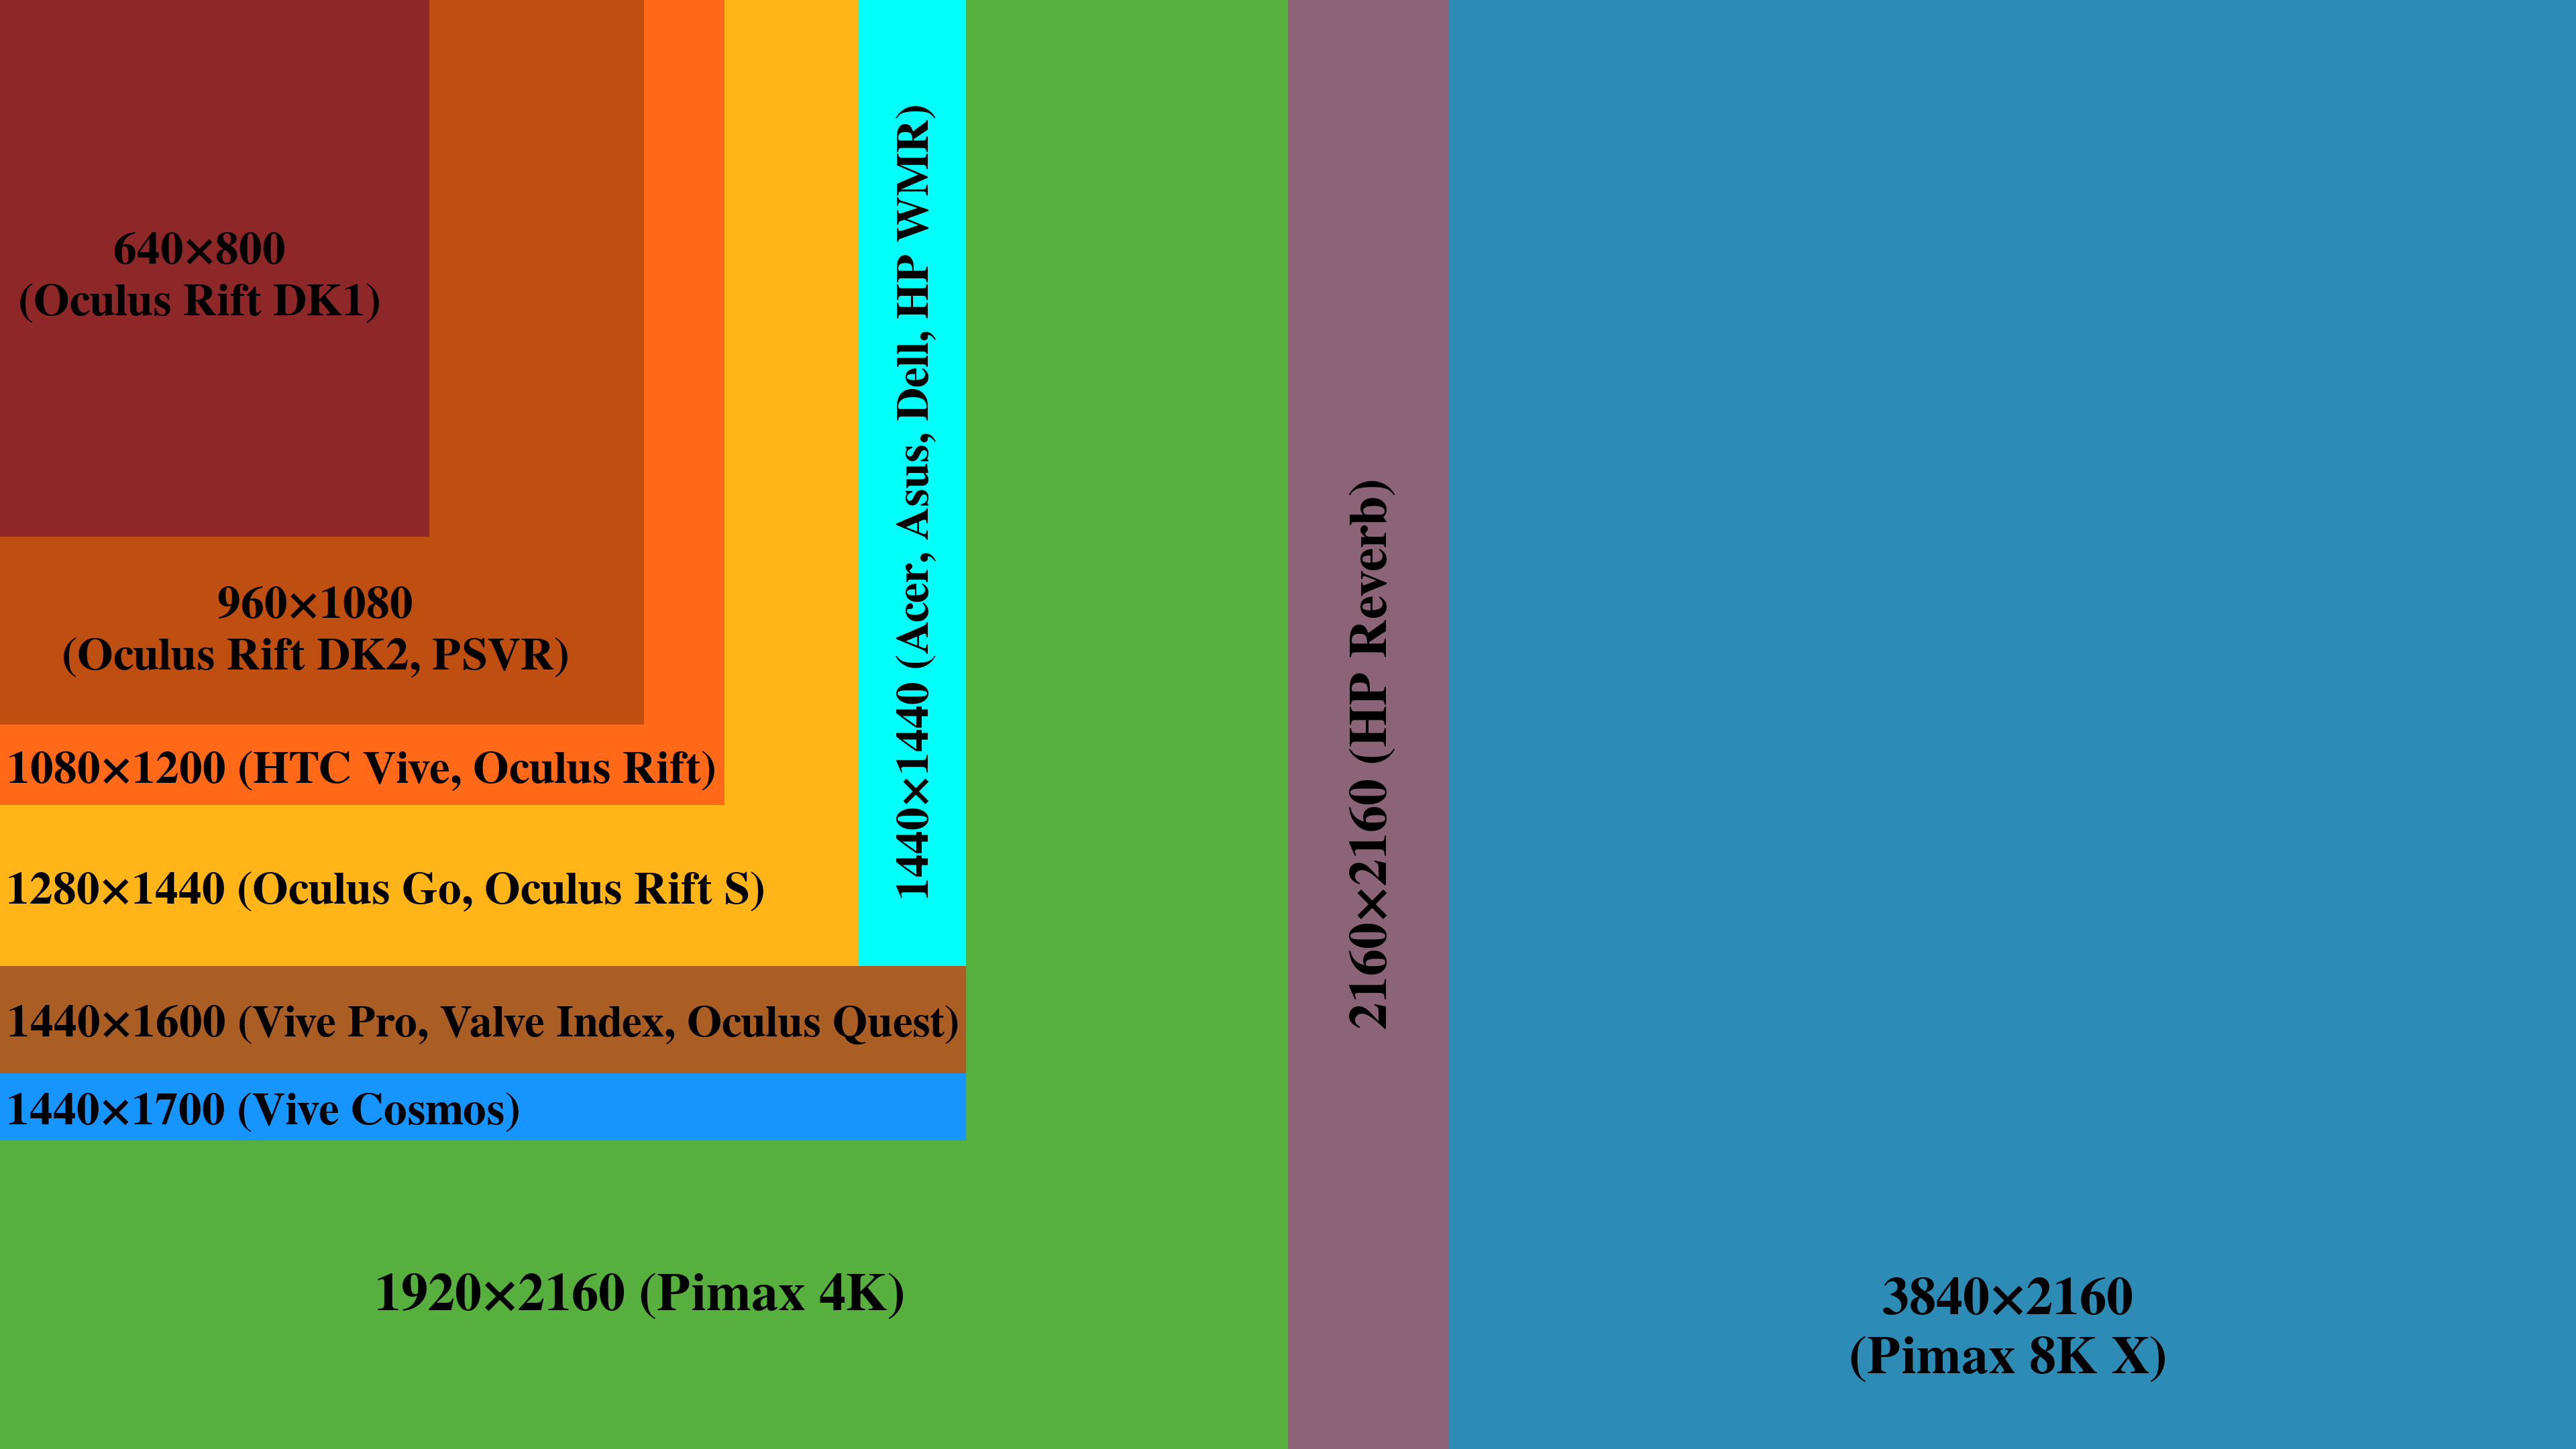
\includegraphics[width=0.9\textwidth]{pictures/VR_headset_resolution_per_eye_comparison}
  \caption{Comparison of common HMD resolutions (Oct 2019)\cite{VeikkoMakela.2019}} \label{fig:VR_HMD_res}
\end{figure} 

\section{The goal}
While this is very rough napkin math and real applications scale differently to a degree due to a multitude of factors, it paints a clear picture: real-time virtual reality rendering necessitates vastly faster rendering than traditional screens. It obviously follows that VR rendering should take advantage of as much optimization as possible to attain that goal. There are many established options that are known to improve performance for various if not most application types, with some of these options being de-facto standard features in popular rendering engines.  There is also, however, a range of optimizations specific to virtual reality or more generally stereoscopic rendering, and often there is less research and documentation available yet, due in part to aforementioned recent rise in popularity and prior lack of interest. \\
Thus, this paper aims to collect several of these VR optimizations, implement a subset of them in a real engine and then benchmark and analyse the impact each has on performance. The goal is to have a better collection and understanding of the various methods to use and how much effort may be warranted for each. 
To this end, what follows is first an explanation of the software and technical foundation used to implement practical samples, a chapter on optimizations aiming to reduce render \textit{input}, succeeded by a chapter on optimizations aiming to reduce render \textit{effort} and finally an analysis of the performance impact of each implemented approach. Note here that only a subset of the listed methods was implemented due to time constraints. 

\section{Industry collaboration}
This thesis is created in collaboration with RTG Echtzeitgraphik GmbH, an engineering and consulting office based in Garching bei München. RTG offers engineering services related to real-time visualization, virtual reality applications and hardware prototyping to enterprise clients from a variety of industry branches such as automotive and industrial logistics\cite{HansiVollmer.2020}. \\
At this point it needs to be disclaimed that the author of this thesis was employed at RTG Echtzeitgraphik GmbH at the time of making. This allowed the use of company assets like workstations, a range of VR headsets and relevant literature as well as expertise with regard to related technologies and enterprise requirements for a rendering engine. The thesis, accompanied research efforts and all material created for the purpose of this thesis, however, are the author's own work. 

\begin{figure}[htb]
  \centering
  
\includegraphics[width=0.5\textwidth]{pictures/RTG_Logo}
\end{figure} 

\section{Technical foundation}
From this industry collaboration follow influences when choosing the technical foundations of the thesis. In an effort to represent a realistic use case, an engine with actual production usage target was chosen as opposed to a purely synthetic "test vehicle", namely RTG's own \textit{Tachyon}. The engine and its structure is further explained in \autoref{Tachyon}. \\
The graphics API and library of choice for this thesis then is the Khronos Group's Vulkan. Vulkan is a low level graphics API officially created in 2014 and formally released in early 2016 with the promise of increased flexibility and reduced overhead compared to prior graphics APIs as well as compatibility with a wide range of hardware architectures and operating systems\cite{TheKhronosGroupInc..2016}. On the flipside, the verbose and low level nature of the API brings increased development effort and means that these promised improvements can only be leveraged with sufficient care and caution by developers. \\
More specifically for \textit{Tachyon} and this thesis, the goal is to enable fast rendering of complex scenes with very large object counts, all while driving virtual reality headsets at high resolution and framerate. Vulkan promises a good fit for this purpose. Furthermore Vulkan is seeing a steady growth in developer interest and industry adoption, but with documentation, resources and API-specific research still being lackluster in some ways. This thesis hopes to add useful insights to this pool. \\
Lastly - as a sort of tease to the future - both Vulkan and the VR optimizations presented here are not just compatible with powerful x86 desktop machines, but also with many ARM-based SoCs running Google's Android as well as Apple's iOS, promising prospects for the category of standalone low power VR headsets which are seeing increasing popularity\cite{AntonyVitillo.2018}\cite{IDCCorporateUSA.2020}. 



\iffalse
\chapter{Prior research [TEMP]}\label{chapter:introduction}

\section{Culling methods research}
\subsection{Assorted sources}
1. Experiments in GPU-based occlusion culling (Anagnostou, Interplay of Light) \cite{Anagnostou.2017}: \\
tldr CPU occlusion culling is very coarse as the CPU isn't great at rasterising. GPU can rasterise efficiently and supports hardware occlusion queries. Problem: "drawcall level" granularity, needs query and fence around every drawcall, thus can't handle instancing very well. Other problem: readback to CPU necessary, to avoid stalling use previous frame occlusion info for current frame. Thus popping likely for fast moving objects or camera. 
Other solution: render low res occlusion buffer on GPU, produce mip chain, determine screen-space size of each prop and compare vs appropriate mip-level of buffer. Still needs CPU readback though, unless... compute shader in modern API: "In this case I will be using a compute shader to perform the occlusion tests, producing a list of visible props that I will then be consuming on the GPU, avoiding the CPU roundtrip."\\

2. Why Frustum Culling Matters, and Why It's Not Important \cite{Barrett.2017}: \\
tldr disregardm, oversimplified explanation of frustum culling.\\

3. Overview on popular occlusion culling techniques \cite{gamesindustry.biz.2016}: \\
tldr temporal culling methods are prone to artifacting with fast object or camera movement, CPU culling "is the most efficient, forward-looking approach", then again the article is written by someone from Umbra3D, a CPU occlusion culling middleware. 
Still, precomputed visibility sets for weak devices are brought up, low res HI-Z depth buffer rasterised on the CPU with SIMD units for dynamic culling, see Intel's 2015/2016 occlusion culling article.\\

4. Frustum Culling \cite{Gerlits.2017}: \\
tldr code samples and brief performance numbers for bounding sphere, AABB, OBB based culling, SSE support, MT support, somewhat simple GPU culling. Sphere or AABB with SSE + MT support quite fast, 0.1-0.2ms for 100k objects on unspecified i5 quadcore.\\

5. Dual-Cone View Culling for Virtual Reality Applications \cite{Hale.2018}: \\
tldr not discernibly faster than frustum pyramid culling plus stencil mesh. Needs careful tuning for each HMD to avoid performing worse when a larger image is rendered and warped to view. With SIMD, more accurate cones etc may be more efficient.\\

6. Culling Techniques \cite{ITCS.Subramanian}: \\
tldr general explanation. Of interest maybe hierarchical bounding volumes for frustum culling. As the goal is a fast rendering of extreme number of objects, hierarchical ordering seems obviously necessary.\\

7. A Survey of Visibility for Walkthrough Applications \cite{CohenOr.2003}: \\
tldr .\\

8. Occlusion Culling Methods \cite{Hey.2001}: \\
tldr overview of methods anno 2001 (duh). Hierarchical frustum culling, occluder fusion, etc.\\

9. Math for Game Developers - Frustum Culling\cite{Rodriguez.2013}: \\
tldr as expected, brief mathematical explanation on how to compute whether a prop is inside the view frustum (based on position and prop radius).\\

10. Wie Sie einen Einstieg in das Frustum Culling finden \cite{VisCircleGmbH.}: \\
tldr D3D sample code for view frustum culling. Very brief, not very useful. But raises the questions how to compute (and store) bounding sphere radius for each prop, and how to compute and update frustum planes each frame (aka reconstruct from view + proj matrices or set up at start and then move all planes according to camera movement).\\

11. Superfrustum culling \cite{Whiting.2017}: \\
tldr instead of one frustum per eye, construct one superfrustum covering both. On paper means somewhat fewer objects are culled, but the reduced overhead still comes out on top. In their testing, shaved off ~1ms on lower end CPUs. Also monoscopic far-field for lower end devices and far draw distances: past a certain distance, stereo separation becomes very small, nigh indistinguishable, so it may be faster to render the far field monoscopic and then composit with the near-field stereo image.\\

12. OpenGL sample for shader-based occlusion culling \cite{Kubisch.2014}: \\
tldr shader-based batched occlusion culling system: leverages multi\char`_draw\char`_indirect and works well with setups where all geo is stored in one big buffer.\\

13. GPU occlusion culling using compute shader with Vulkan \cite{sydneyzh.2018}: \\
tldr follows \cite{Anagnostou.2017} to showcase GPU occlusion culling.\\

14. Understanding Culling Methods | Live Training | Unreal Engine \cite{Hobson.2019}: \\
tldr basic explanation of methods employed in UE4.\\

More:\\
15. Occlusion Culling Algorithms \cite{Haines.1999}. \\
16. View Frustum Culling \cite{Lighthouse3d.com.2011}.\\
17. How Occlusion Culling Works \cite{thebennybox.2018}.\\
18. Cull and LOD: Compute shader culling and LOD using indirect rendering \cite{Willems.2016.6}.\\
19. Occlusion queries: Using occlusion query for visibility testing \cite{Willems.2016.4}.\\
20. Visibility and Occlusion Culling \cite{EpicGamesInc..n.d.}.\\

\subsection{Other conference talks}
21. Advanced VR Rendering with Valve's Alex Vlachos (GDC'15) \cite{Vlachos.2016}.\\
22. Advanced VR Rendering (GDC'16) \cite{Vlachos.2016b}.\\
23. Practical Development for Vulkan (GDC'16) \cite{Ginsburg.2016}.\\
24. Fast and Flexible: Technical Art and Rendering for The Unknown (VRDC'16) \cite{Answer.2016}.\\
25. Bringing Vulkan to VR (DevU'17) \cite{Everitt.2017}.\\

\subsection{Culling aspects worth looking at}
\textbf{Thus, things up in the air: }\\
CPU-based: (hierarchical/chunk-based) frustum culling, occlusion culling (e.g. mipped depth raster) and front-to-back ordering, detail culling (e.g. size-distance function or center-distance culling of peripheral objects), simple distance culling\\
GPU-based: same, really, but shader/compute based (However, I have a lot of respect for these approaches as GPU-based culling is a whole other beast. I would prefer to stick with CPU-based approaches for starters.)\\
Specifically for frustum culling: dual-view frustum culling vs superfrustum culling evaluation\\
General: stencil meshing, SIMD and MT optimization

\section{Another angle: Monoscopic far-field rendering}
Slides 14-31 in \cite{DiDonato.01.03.2017}, \cite{EpicGamesInc..2016} and \cite{FacebookTechnologiesLLC..2016}: Basic idea is to render near-field (e.g. first 30ft) in stereo for good separation effect, anything beyond that in mono, then mask the background and composite the two images. This leverages the fact that stereo separation becomes very minimal beyond a certain distance, even so small that it's less than 1px shift. When tuned correctly and used in scenes with many objects beyond the threshold distance, this can yield good performance improvements of up to 25\%. The savings from only drawing far objects once must outweigh the cost of adding another camera and more render passes. 
Another question is how savings scale when multiview rendering is used, as it already avoids a lot of redundant vertex shader work. 
While Epic Games seem to have dropped the feature from Unreal Engine in 4.22 for yet unknown reasons, I couldn't find much further research about it. 
One curious extension would be to use the far-field depth buffer to shift the image slightly in post-processing to create a fake stereo separation effect. Or perhaps to render not a centered far-field image, but to use the far-field image of each eye in alternating fashion. This may allow a further reduction in near-field far plane while still being a convincing approximation. 

\section{Research during implementation and testing}
GPU Zen 1, 2\\
Intel Software, Masked Occlusion Culling\\

\section{Renderer current status}
\begin{itemize}
\item using Vulkan 1.1.97+ and OpenVR 1.4.18 
\item using RTG's rtvklib rendering library and wx-vk UI library, both still in development
\item available rendering features: 
\begin{itemize}
\item VK\char`_multiview based stereo rendering 
\item pipelines for blinn-phong shading, PBR shading, skybox
\item OpenVR roomscale tracking 
\item assets supported in in-house .hvr format
\end{itemize}
\item so far tested successfully with Valve Index, HTC Vive and Vive Pro, Samsung Odyssey 
\item rendering features to be ported from discontinued Valkun project: 
\begin{itemize}
\item VR stencil mesh mask
\item OpenVR rendermodel readout 
\end{itemize}
\end{itemize}
\fi



\iffalse
\subsection{Subsection}

See~\autoref{tab:sample}, \autoref{fig:sample-drawing}, \autoref{fig:sample-plot}, \autoref{fig:sample-listing}, \autoref{fig:tum}, \autoref{fig:tumslide}.

\begin{table}[htpb]
  \caption[Example table]{An example for a simple table.}\label{tab:sample}
  \centering
  \begin{tabular}{l l l l}
    \toprule
      A & B & C & D \\
    \midrule
      1 & 2 & 1 & 2 \\
      2 & 3 & 2 & 3 \\
    \bottomrule
  \end{tabular}
\end{table}

\begin{figure}[htpb]
  \centering
  % This should probably go into a file in figures/
  \begin{tikzpicture}[node distance=3cm]
    \node (R0) {$R_1$};
    \node (R1) [right of=R0] {$R_2$};
    \node (R2) [below of=R1] {$R_4$};
    \node (R3) [below of=R0] {$R_3$};
    \node (R4) [right of=R1] {$R_5$};

    \path[every node]
      (R0) edge (R1)
      (R0) edge (R3)
      (R3) edge (R2)
      (R2) edge (R1)
      (R1) edge (R4);
  \end{tikzpicture}
  \caption[Example drawing]{An example for a simple drawing.}\label{fig:sample-drawing}
\end{figure}

\begin{figure}[htpb]
  \centering

  \pgfplotstableset{col sep=&, row sep=\\}
  % This should probably go into a file in data/
  \pgfplotstableread{
    a & b    \\
    1 & 1000 \\
    2 & 1500 \\
    3 & 1600 \\
  }\exampleA
  \pgfplotstableread{
    a & b    \\
    1 & 1200 \\
    2 & 800 \\
    3 & 1400 \\
  }\exampleB
  % This should probably go into a file in figures/
  \begin{tikzpicture}
    \begin{axis}[
        ymin=0,
        legend style={legend pos=south east},
        grid,
        thick,
        ylabel=Y,
        xlabel=X
      ]
      \addplot table[x=a, y=b]{\exampleA};
      \addlegendentry{Example A};
      \addplot table[x=a, y=b]{\exampleB};
      \addlegendentry{Example B};
    \end{axis}
  \end{tikzpicture}
  \caption[Example plot]{An example for a simple plot.}\label{fig:sample-plot}
\end{figure}

\begin{figure}[htpb]
  \centering
  \begin{tabular}{c}
  \begin{lstlisting}[language=SQL]
    SELECT * FROM tbl WHERE tbl.str = "str"
  \end{lstlisting}
  \end{tabular}
  \caption[Example listing]{An example for a source code listing.}\label{fig:sample-listing}
\end{figure}

\begin{figure}[htpb]
  \centering
  \includegraphics[width=0.8\textwidth]{tum}
  \caption[Something else can be written here for listing this, otherwise the caption will be written!]{Includegraphics searches for the filename without extension first in logos, then in figures.} \label{fig:tum}
\end{figure}

\begin{figure}[htpb]
  \centering
  \includegraphics[width=0.8\textwidth]{figures/tum}
  \caption{For pictures with the same name, the direct folder needs to be chosen.} \label{fig:tumslide}
\end{figure}

\begin{figure}[!tbp]
  \centering
  \subfloat[TUM Logo][The logo.]{\includegraphics[height=0.2\textheight]{tum}\label{fig:tum1}}
  \hfill
  \subfloat[TUM Slide][The famous slide.]{\includegraphics[height=0.2\textheight]{figures/tum}\label{fig:tum2}}
  \caption{Two TUM pictures side by side.}
  \label{fig:sidebyside}
\end{figure}

This is how the glossary will be used.

\Glspl{ddye}, \gls{r0}, \gls{R0}, and \gls{kdeac}. Also, the \glspl{tum} has many \glspl{computer}, not only one \Gls{computer}. Subsequent acronym usage will only print the short version of \glspl{tuma} (take care of plural, if needed!), like here with \gls{tuma}, too. It can also be --> \glsdisp{tum}{hidden}\footnote{Example for a hidden TUM glossary entry.} <--.

\todo{Now it is your turn to write your thesis.

This will be a few tough weeks.}

\done{Nevertheless, celebrate it when it is done!}
\fi
